
\de{ĐỀ THI HỌC KỲ I NĂM HỌC 2022-2023}{Trường THPT Hùng Vương - Quảng Nam}
\begin{center}
	\textbf{PHẦN 1 - TRẮC NGHIỆM}
\end{center}
\Opensolutionfile{ans}[ans/ans]
%Câu 1...........................
\begin{ex}%[0H2B2-1]%[Dự án đề kiểm tra HKII NH22-23- Huỳnh Quy]%[Trường THPT Hùng Vương - Quảng Nam]
	Cho hình bình hành $ABCD$. Véc-tơ tổng $\vec{CB}+\vec{CD}$ bằng
	\choice
	{\True $\vec{CA}$}
	{$\vec{BD}$}
	{$\vec{AC}$}
	{$\vec{DB}$}
	\loigiai{
	Theo quy tắc hình bình hành, ta có 	$\vec{CB}+\vec{CD}=\vec{CA}$. 
	}
\end{ex}
\begin{ex}%[0H3B1-3]%[Dự án đề kiểm tra HKII NH22-23- Huỳnh Quy]%[Trường THPT Hùng Vương - Quảng Nam]
	Trong mặt phẳng tọa độ $Oxy$, cho $A(4;2)$, $B(1;-5)$. Tìm tọa độ trọng tâm $G$ của tam giác $OAB$.
	\choice
	{$G\left(\dfrac{5}{3};\dfrac{1}{3}\right)$}
	{$G\left(\dfrac{5}{2};2\right)$}
	{$G\left(1;3\right)$}
	{\True $G\left(\dfrac{5}{3};-1\right)$}
	\loigiai{
	Gọi $G(x_G;y_G)$. Ta có
	\[
	\heva{	&x_G=\dfrac{x_A+x_B+x_O}{3}=\dfrac{4+1+0}{3}=\dfrac{5}{3}\\
			&y_G=\dfrac{y_A+y_B+y_O}{3}=\dfrac{2+(-5)+0}{3}=\dfrac{-3}{3}=-1.}\Rightarrow G\left(\dfrac{5}{3};-1\right).
	\]	
	}
\end{ex}
\begin{ex}%[0H3B2-1]%[Dự án đề kiểm tra HKII NH22-23- Huỳnh Quy]%[Trường THPT Hùng Vương - Quảng Nam]
	Cho hai véc-tơ $\vec{u}=(2;3)$, $\vec{v}=(0;5)$. Tích $\vec{u}\cdot\vec{v}$ bằng
	\choice
	{$11$}
	{$-10$}
	{\True $15$}
	{$-2$}
	\loigiai{
	Ta có $\vec{u}\cdot\vec{v}=2\cdot 0+3\cdot 5=15$.
	}
\end{ex}

\begin{ex}%[0H3B2-2]%[Dự án đề kiểm tra HKII NH22-23- Huỳnh Quy]%[Trường THPT Hùng Vương - Quảng Nam]
	Trong mặt phẳng tọa độ $Oxy$, cho hai véc-tơ $\vec{a}=(4;3)$ và $\vec{b}=(1;7)$. Góc $\alpha$ giữa hai véc-tơ $\vec{a}$ và $\vec{b}$ bằng
	\choice
	{$\alpha=90^{\circ}$}
	{\True $\alpha=45^{\circ}$}
	{$\alpha=60^{\circ}$}
	{$\alpha=30^{\circ}$}
	\loigiai{
	Ta có $\cos\alpha=\dfrac{\vec{a}\cdot\vec{b}}{|\vec{a}|\cdot|\vec{b}|}=\dfrac{4\cdot 1+3\cdot 7}{\sqrt{4^2+3^2}\cdot\sqrt{1^2+7^2}}=\dfrac{25}{5\cdot 5\sqrt{2}}=\dfrac{\sqrt{2}}{2}\Rightarrow\alpha=45^{\circ}$.
	}
\end{ex}
\begin{ex}%[0H2K4-3]%[Dự án đề kiểm tra HKII NH22-23- Huỳnh Quy]%[Trường THPT Hùng Vương - Quảng Nam]
	Cho tam giác $ABC$. Khẳng định nào sau đây \textbf{đúng}?
	\choice
	{\True $S=\dfrac{1}{2}AC\cdot AB\cdot\sin A$}
	{$S=\dfrac{1}{2}BC\cdot AB\cdot \sin A$}
	{$S=\dfrac{1}{2}AC\cdot AB\cdot\sin B$}
	{$S=\dfrac{1}{2}BC\cdot AB\cdot \sin C$}
	\loigiai{
	Công thức đúng là $S=\dfrac{1}{2}AC\cdot AB\cdot\sin A$.
	}
\end{ex}
\begin{ex}%[0H2B1-3]%[Dự án đề kiểm tra HKII NH22-23- Huỳnh Quy]%[Trường THPT Hùng Vương - Quảng Nam]
	Cho hình bình hành $MNPQ$. Khẳng định nào sau đây \textbf{sai}?
	\choice
	{$\left|\vec{MN}\right|=\left|\vec{PQ}\right|$}
	{\True $\vec{MQ}=\vec{PN}$}
	{$\vec{MN}=\vec{QP}$}
	{$\left|\vec{MQ}\right|=\left|\vec{PN}\right|$}
	\loigiai{
	\immini{Dễ thấy $\vec{MQ}=\vec{NP}$. Do đó khẳng định ``$\vec{MQ}=\vec{PN}$'' là khẳng định sai.}{\begin{tikzpicture}
			\coordinate (M) at (0,0);
			\coordinate (N) at (4,0);
			\coordinate (Q) at (3,2);
			\coordinate (P) at ($(N)+(Q)-(M)$);
			\draw (M)--(N)--(P)--(Q)--cycle;
			\foreach \x in {M,N,P,Q}\draw[fill=red] (\x) circle (2pt);
			\foreach \x in{M,N} \draw (\x) node[below]{$\x$};
			\foreach \x in{P,Q} \draw (\x) node[above]{$\x$};
	\end{tikzpicture}}	
	}
\end{ex}

\begin{ex}%[0H2B2-1]%[Dự án đề kiểm tra HKII NH22-23- Huỳnh Quy]%[Trường THPT Hùng Vương - Quảng Nam]
	Cho hình bình hành $MNPQ$. Mệnh đề nào dưới đây \textbf{đúng}?
	\choice
	{\True $\vec{MN}+\vec{MQ}=\vec{MP}$}
	{$\vec{MN}+\vec{MQ}=\vec{PQ}$}
	{$\vec{MN}+\vec{MQ}=\vec{NQ}$}
	{$\vec{MN}+\vec{MQ}=\vec{NQ}$}
	\loigiai{
	\immini{Khẳng định đúng là ``$\vec{MN}+\vec{MQ}=\vec{MP}$'' (quy tắc hình bình hành).}{\begin{tikzpicture}
			\coordinate (M) at (0,0);
			\coordinate (N) at (4,0);
			\coordinate (Q) at (3,2);
			\coordinate (P) at ($(N)+(Q)-(M)$);
			\draw (M)--(N)--(P)--(Q)--cycle;
			\foreach \x in {M,N,P,Q}\draw[fill=red] (\x) circle (2pt);
			\foreach \x in{M,N} \draw (\x) node[below]{$\x$};
			\foreach \x in{P,Q} \draw (\x) node[above]{$\x$};
			\draw[->] (M)--(N) (M)--(Q) (M)--(P);
	\end{tikzpicture}}
	}
\end{ex}
\begin{ex}%[0H2B2-3]%[Dự án đề kiểm tra HKII NH22-23- Huỳnh Quy]%[Trường THPT Hùng Vương - Quảng Nam]
	Cho đoạn thẳng $AB$. Điều kiện cần và đủ để điểm $I$ là trung điểm của đoạn thẳng $AB$ là
	\choice
	{$IA=IB$}
	{$\vec{AI}=\vec{BI}$}
	{$AB=2AI$}
	{\True $\vec{IA}+\vec{IB}=\vec{0}$}
	\loigiai{
	Điều kiện cần và đủ để điểm $I$ là trung điểm của đoạn thẳng $AB$ là $\vec{IA}+\vec{IB}=\vec{0}$.
	}
\end{ex}

\begin{ex}%[0H3B1-1]%[Dự án đề kiểm tra HKII NH22-23- Huỳnh Quy]%[Trường THPT Hùng Vương - Quảng Nam]
	Trên mặt phẳng với hệ tọa độ $Oxy$, cho véc-tơ $\vec{u}=2022\vec{i}-2023\vec{j}$. Tọa độ của véc-tơ $\vec{u}$ là
	\choice
	{$\vec{u}=(-2022;-2023)$}
	{$\vec{u}=(2022;2023)$}
	{\True $\vec{u}=(2022;-2023)$}
	{$\vec{u}=(-2022;2023)$}
	\loigiai{
	Ta có $\vec{u}=2022\vec{i}-2023\vec{j}=(2022;-2023)$.
	}
\end{ex}

\begin{ex}%[0H3B1-1]%[Dự án đề kiểm tra HKII NH22-23- Huỳnh Quy]%[Trường THPT Hùng Vương - Quảng Nam]
	Trên mặt phẳng với hệ tọa độ $Oxy$, cho $A(10;0)$, $B(0;2022)$. Tọa độ trung điểm $I$ của đoạn thẳng $AB$ là
	\choice
	{$I(5;-1011)$}
	{$I(-5;1011)$}
	{$I(-10;2022)$}
	{\True $I(5;1011)$}
	\loigiai{
	Gọi $I(x_I;y_I)$. Ta có
	\[
	\heva{&x_I=\dfrac{x_A+x_B}{2}=\dfrac{10+0}{2}=5\\&y_I=\dfrac{y_A+y_B}{2}=\dfrac{0+2022}{2}=1011}\Rightarrow I(5;1011).
	\]	
	}
\end{ex}
\begin{ex}%[0D1B1-2]%[Dự án đề kiểm tra HKII NH22-23- Huỳnh Quy]%[Trường THPT Hùng Vương - Quảng Nam]
	Kí hiệu nào sau đây dùng để viết đúng mệnh đề ``$\sqrt{2}$ không phải là số hữu tỉ''?
	\choice
	{$\sqrt{2}\notin \mathbb{Q}$}
	{$\sqrt{2}\not\subset\mathbb{Q}$}
	{\True $\sqrt{2}\notin\mathbb{Q}$}
	{$\sqrt{2}\in\mathbb{Q}$}
	\loigiai{
	Kí hiệu đúng là ``$\sqrt{2}\notin \mathbb{Q}$''.	
	}
\end{ex}

\begin{ex}%[0D1B2-2]%[Dự án đề kiểm tra HKII NH22-23- Huỳnh Quy]%[Trường THPT Hùng Vương - Quảng Nam]
	Cho tập hợp $A=\{1;2;3;4\}$. Số tập hợp con gồm hai phần tử của tập hợp $A$ là
	\choice
	{$4$}
	{$8$}
	{$16$}
	{\True $6$}
	\loigiai{
	Các tập con gồm $2$ phần tử của tập $A$ là $\{1;2\}$; $\{1;3\}$; $\{1;4\}$;$\{2;3\}$; $\{2;4\}$; $\{3;4\}$. Vậy có $6$ tập con thỏa mãn yêu cầu bài toán.
	}
\end{ex}
\begin{ex}%[0D2B1-1]%[Dự án đề kiểm tra HKII NH22-23- Huỳnh Quy]%[Trường THPT Hùng Vương - Quảng Nam]
	Bất phương trình nào sau đây là bất phương trình bậc nhất hai ẩn $x$, $y$?
	\choice
	{\True $\sqrt{3}x-y<5^2$}
	{$x^2+3y<4$}
	{$\sqrt{2}x-5xy>0$}
	{$x+3y+z-xyz<0$}
	\loigiai{
	Bất phương trình bậc nhất hai ẩn $x$, $y$ là ``$\sqrt{3}x-y<5^2$''.	
	}
\end{ex}

\begin{ex}%[0D2B2-2]%[Dự án đề kiểm tra HKII NH22-23- Huỳnh Quy]%[Trường THPT Hùng Vương - Quảng Nam]
	Miền nghiệm của hệ bất phương trình $\heva{&\dfrac{x}{2}+\dfrac{y}{3}-1\geq 0\\&x\geq 0\\&x+\dfrac{1}{2}-\dfrac{3y}{2}\leq 2}$ chứa điểm nào trong các điểm sau đây?
	\choice
	{$O(0;0)$}
	{$N(1;1)$}
	{\True $M(2;1)$}
	{$P(5;1)$}
	\loigiai{
	Ta lần lượt thay tọa độ các điểm $M$, $N$, $P$, $Q$ vào từng bất phương trình của hệ đã cho, chỉ có điểm $M(2;1)$ thỏa mãn.	
	}
\end{ex}

\begin{ex}%[1D1B2-2]%[Dự án đề kiểm tra HKII NH22-23- Huỳnh Quy]%[Trường THPT Hùng Vương - Quảng Nam]
	Cho $\alpha$ và $\beta$ là hai góc khác nhau và bù nhau, trong các đẳng thức sau đây đẳng thức nào \textbf{sai}?
	\choice
	{$\sin\alpha=\sin\beta$}
	{$\cos\alpha=-\cos\beta$}
	{$\tan\alpha=-\tan\beta$}
	{\True $\cot\alpha=\cot\beta$}
	\loigiai{
	Hai góc bù nhau thì chỉ có giá trị $\sin$ bằng nhau, tức là $\sin \alpha=\sin\beta$, còn lại đối nhau.\\
	Do đó, khẳng định ``$\cot\alpha=\cot\beta$'' là khẳng định sai.
	}
\end{ex}


\Closesolutionfile{ans}
%\begin{center}
%	\textbf{ĐÁP ÁN}
%	\inputansbox{10}{ans/ans}	
%\end{center}
\begin{center}
	\textbf{PHẦN 2 - TỰ LUẬN}
\end{center}

%Cau1
\begin{bt}%[0D1Y2-3]%[0D1B3-1]%[Dự án đề kiểm tra HKII NH22-23- Phan Trung Hiếu]%[THPT Hùng Vương - Quảng Nam]
	Cho hai tập hợp $A=[1;4]$ và $B=(3;6)$.
	\begin{enumerate}
		\item Biểu diễn tập $A$ và tập $B$ trên từng trục số.
		\item Xác định các tập hợp $A\cup B$, $A\cap B$. 
	\end{enumerate}
\loigiai{
\begin{enumerate}
	\item Tập hợp $A$
	\begin{center}
		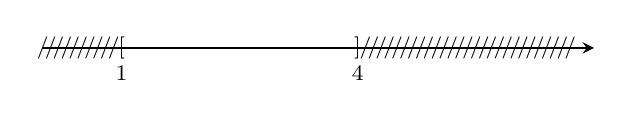
\begin{tikzpicture}[font=\footnotesize, line cap=round, line join=round, thick]
			\node at (1,0) {$[$};
			\node at (4,0) {$]$};
			\draw[-stealth] (0,0)--(1,0)node[below=3pt]{$1$}--(4,0)node[below=3pt]{$4$}--(7,0);
			\foreach \x in {0,.1,.2,...,.9}
				\draw (\x,0)node{$/$};
			\foreach \y in {4.1,4.2,...,6.7}
				\draw (\y,0)node{$/$};
		\end{tikzpicture}
	\end{center}
			Tập hợp $B$
	\begin{center}
		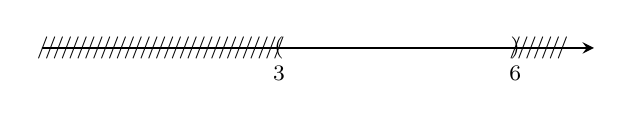
\begin{tikzpicture}[font=\footnotesize, line cap=round, line join=round, thick]
			\node at (3,0) {$($};
			\node at (6,0) {$)$};
			\draw[-stealth] (0,0)--(3,0)node[below=3pt]{$3$}--(6,0)node[below=3pt]{$6$}--(7,0);
			\foreach \x in {0,.1,.2,...,3}
			\draw (\x,0)node{$/$};
			\foreach \y in {6,6.1,...,6.7}
			\draw (\y,0)node{$/$};
		\end{tikzpicture}
	\end{center}
	\item $A\cup B = [1;6)$, $A\cap B= (3;4]$.
\end{enumerate}
}
\end{bt}
%Cau2
\begin{bt}%[0H2B2-4]%[Dự án đề kiểm tra HKII NH22-23- Phan Trung Hiếu]%[THPT Hùng Vương - Quảng Nam]
	Cho tam giác $ABC$. Xác định vị trí điểm $M$ trong mặt phẳng chứa $\triangle ABC$ sao cho $\vv{MA}=\vv{MC}-\vv{MB}$ (có vẽ hình minh họa vị trí điểm $M$).
	\loigiai{
	Ta có $\vv{MA}=\vv{MC}-\vv{MB}\Leftrightarrow\vv{MA}=\vv{BC}$ hay $\vv{AM}=\vv{CB}$. Suy ra $M$ là đỉnh của hình bình hành $ACBM$.
	\begin{center}
		\begin{tikzpicture}[font=\footnotesize, thick]
			\path 
			(0,0) coordinate (B)
			(4,0) coordinate (C)
			(1,2) coordinate (A)
			($(A)+(B)-(C)$) coordinate (M)
			;
			\draw (A)--(B)--(C)--cycle;
			\draw[-stealth, >=latex] (A)--(M);
			\foreach \x/\g in {A/90,B/180,C/0,M/90}
			\fill[black] 	(\x) circle (1pt)
			($(\g:3mm)+(\x)$) node {$\x$};
		\end{tikzpicture}
	\end{center}
	}
\end{bt}
%Cau3
\begin{bt}%[0H1Y1-2]%[0H1B2-2]%[Dự án đề kiểm tra HKII NH22-23- Phan Trung Hiếu]%[THPT Hùng Vương - Quảng Nam]
	Cho tam giác $ABC$ có các cạnh $b=6$ (cm), $c=7$ (cm) và $\cos A=\dfrac{3}{4}$.
	\begin{enumerate}
		\item Tính $\sin A$.
		\item Tính diện tích tam giác $ABC$.
	\end{enumerate}
	\loigiai{
	\begin{enumerate}
		\item Ta có $\sin^2A+\cos^2A=1\Rightarrow\sin A=\sqrt{1-\cos^2 A} = \sqrt{1-\dfrac{9}{16}}=\sqrt{\dfrac{7}{16}}=\dfrac{\sqrt{7}}{4}$.
		\item $S_{\triangle ABC}=\dfrac{1}{2}\cdot b\cdot c\cdot\sin A=\dfrac{1}{2}\cdot6\cdot7\cdot\dfrac{\sqrt{7}}{4}=\dfrac{21\sqrt{7}}{4}$ $(\textrm{cm}^2)$.
	\end{enumerate}
	}
\end{bt}
%Cau4
\begin{bt}%[0H2B2-3]%[Dự án đề kiểm tra HKII NH22-23- Phan Trung Hiếu]%[THPT Hùng Vương - Quảng Nam]
	Cho tứ giác $ABCD$. Chứng minh rằng $\vv{AC}+\vv{BD}=\vv{BC}+\vv{AD}$.
	\loigiai{
	Ta có
	\begin{equation*}
		\vv{AC}+\vv{BD} = \vv{AD}+\vv{DC}+\vv{BC}+\vv{CD}=(\vv{AD}+\vv{BC})+(\vv{DC}+\vv{CD}) = \vv{AD}+\vv{BC}+\vec{0} = \vv{BC}+\vv{AD}.
	\end{equation*}
	}
\end{bt}
%Cau5
\begin{bt}%[0H2K4-4]%[Dự án đề kiểm tra HKII NH22-23- Phan Trung Hiếu]%[THPT Hùng Vương - Quảng Nam]
	Trong mặt phẳng với hệ tọa độ $Oxy$, cho $A(1;2)$, $B(-3;4)$ và $C(0;-1)$. Tìm tọa độ điểm $D$ là hình chiếu vuông góc của điểm $A$ trên đường thẳng đi qua hai điểm $B$ và $C$?
	\loigiai{
	Tọa độ điểm $D$ là hình chiếu vuông góc của điểm $A$ trên đường thẳng đi qua hai điểm $B$ và $C$ khi và chỉ khi $\vv{AD}\cdot\vv{BC}=0$ và $\vv{CD}$; $\vv{BC}$ cùng phương.\\
	Khi đó, ta có
	\begin{equation*}
		\heva{&3x-5y=-7\\&5x+3y=-3}\Leftrightarrow\heva{&x=-\dfrac{18}{17}\\&y=\dfrac{13}{17}.}
	\end{equation*}
	trong đó, $\vv{AD} = (x-1;y-2)$, $\vv{BC}=(3;-5)$, $\vv{CD}=(x;y+1)$.
	}
\end{bt}